\chapter{Fundamentos de eletromagnetismo}\label{sec.fund_eletr}

\section{Introdução}

\section{Fatos experimentais}

\subsection{Lei de Gauss para os fluxos elétrico e magnético}\label{sec.lei_gauss}
De acordo com \cite{jackson_classical_1999} e \cite{sommerfeld_52} , os conceitos, definições e resultados em eletromagnetismo clássico partem das experiências de Cavendish e Coulomb no final do Séc. $XVIII$. A partir desses experimentos foi estabelecida a Lei de Coulomb
\begin{equation}\label{eq.forc_elet}
\textbf{F}=k\,\frac{q_1\,q_2}{||\textbf{x}_1-\textbf{x}_2||^2}\frac{\textbf{x}_1-\textbf{x}_2}{||\textbf{x}_1-\textbf{x}_2||},
\end{equation}
onde $q_i$ são as cargas elétricas (campos escalares) presentes nos pontos $\textbf{x}_i$, respectivamente, $k$ (campo escalar) é uma constante de proporcionalidade cujo valor depende do sistema de unidades de medida adotado, $||\textbf{x}_1-\textbf{x}_2||^2$ é a distância Euclidiana entre as cargas e $\textbf{F}$ é a força elétrica exercida pela carga $q_1$ sobre a carga $q_2$. As notações em negrito representam campos vetorias pertencentes ao espaço $\mathbb{R}^3$, e o vetor normal que fornece a direção de interação entre as cargas é dado por $(\textbf{x}_1-\textbf{x}_2)/||\textbf{x}_1-\textbf{x}_2||$.

O campo elétrico $\textbf{E}$ é definido como sendo a força elétrica por unidade de carga em um determinado ponto que contém a carga de prova $q_2$, portanto é uma função vetorial que depende da posição da carga de prova em relação à carga fonte $q_1$, ou seja,
\begin{equation}\label{eq.camp_elet}
\textbf{E}=\lim_{q_2\to 0}\frac{\textbf{F}}{q_2}.
\end{equation}
A carga de prova foi tomada infinitesimalmente pequena para que o campo gerado por ela não perturbe a carga fonte. Experimentalmente, tanto a direção da força como a razão entre a força e a quantidade de carga vão se tornando constantes à medida que a quantidade de carga se torna cada vez menor, definindo a magnitude e a direção do campo elétrico. No SI, a unidade de medida de carga é o \textit{coulomb} $(C)$, o campo elétrico é o \textit{newton/coulomb} $(N/C)$ ou o \textit{volt/metro} $(V/m)$, e a constante $k=(4\pi\,\epsilon_0)^{-1}$ onde $\epsilon_0\simeq8.854\times10^{-12}$ é a \textit{permissividade elétrica no vácuo} medida em \textit{farad/m} $(F/m)$.

Substituindo a equação \ref{eq.camp_elet} em \ref{eq.forc_elet} temos que o campo elétrico agindo num ponto $\textbf{x}$ qualquer devido a uma carga $q_1$ no ponto $\textbf{x}_1$ é
\begin{equation}\label{eq.campo_eletrico}
\textbf{E}=k\,\frac{q_1}{||\textbf{x}_1-\textbf{x}||^2}\frac{\textbf{x}_1-\textbf{x}}{||\textbf{x}_1-\textbf{x}||},
\end{equation}
como podemos observar na figura \ref{fig.camp_eletr} simulando um sistema de coordenadas qualquer.
\begin{figure}[!htb]
\centering
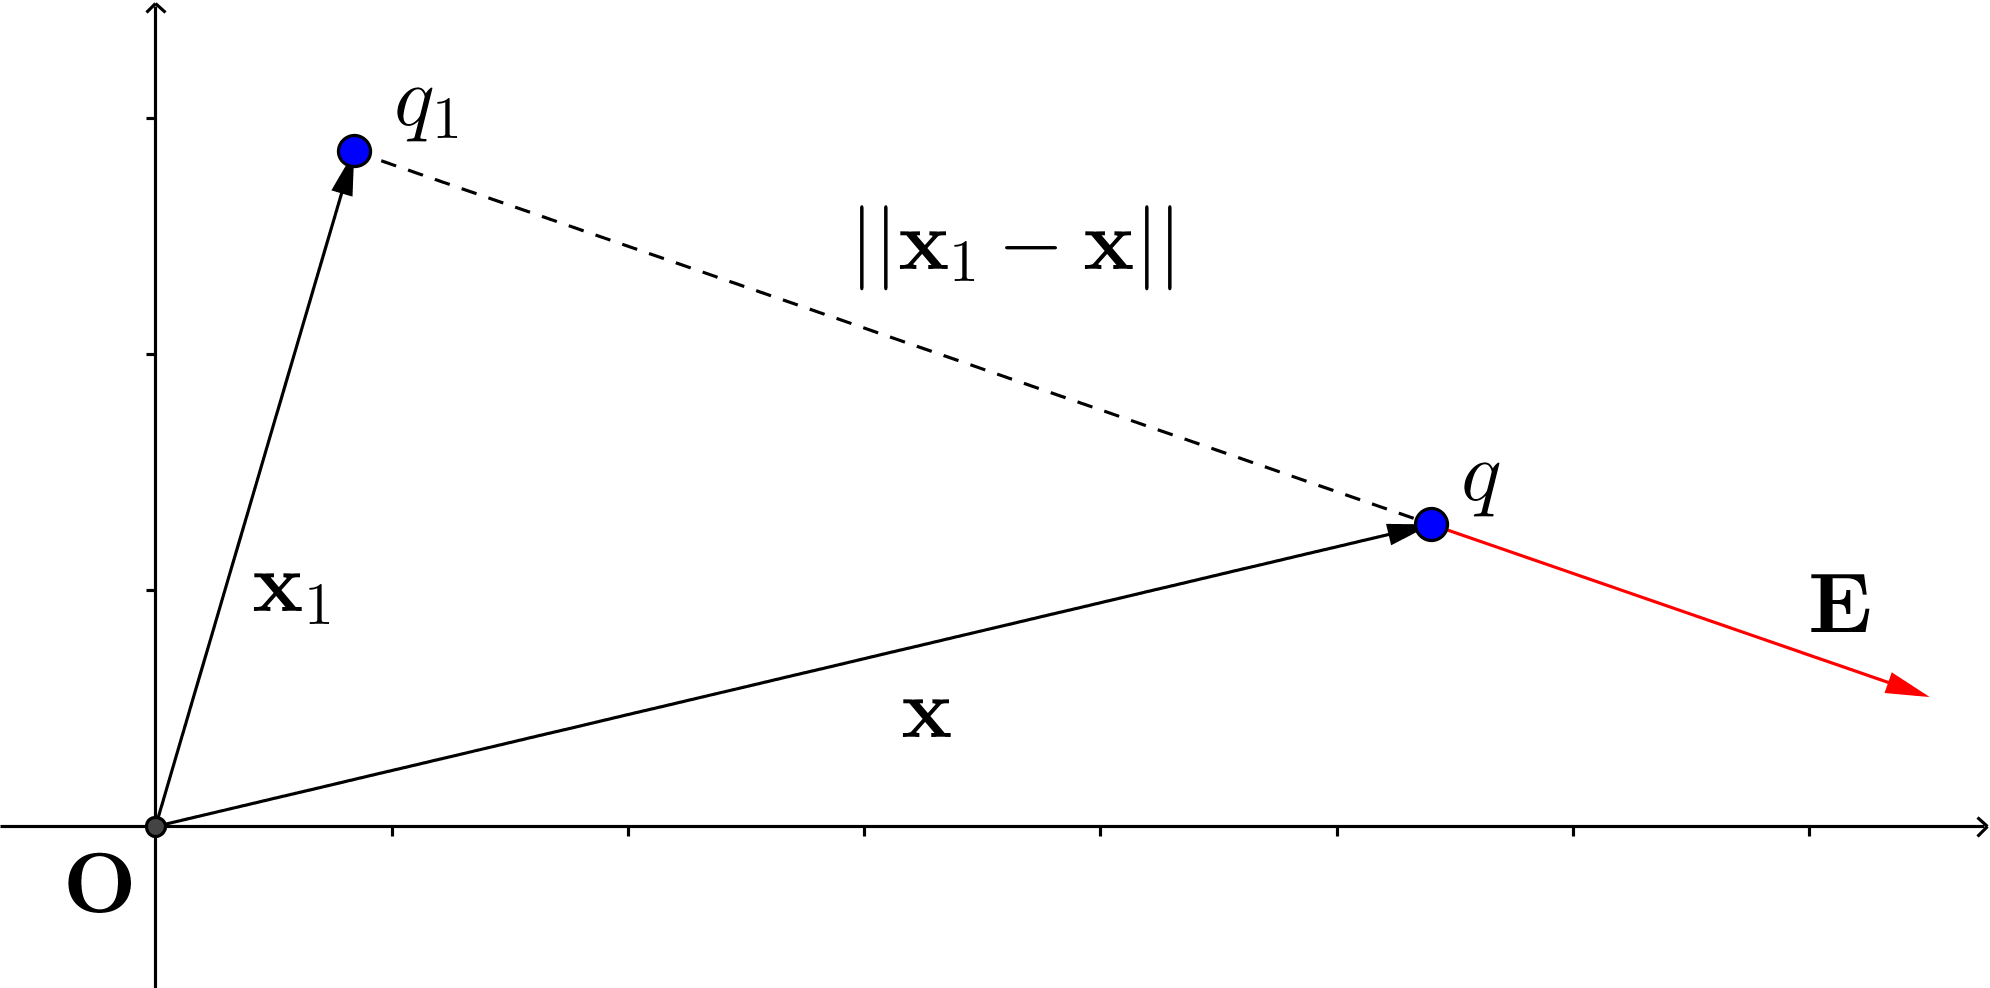
\includegraphics[scale=1.5]{camp_elet}
\caption{\textit{Exemplificação da interação entre cargas elétricas devido à geração, em função de $q_1$ (positiva), de um campo elétrico. A força elétrica $\textbf{F}$ atuando numa carga qualquer $q$ tem mesma direção do campo elétrico $\textbf{E}$, com mesmo sentido ou sentido oposto conforme a carga $q$ é positiva ou negativa, respectivamente.}}
\label{fig.camp_eletr}
\end{figure}

%\begin{figure}[!htb]
%\centering
%\subfloat{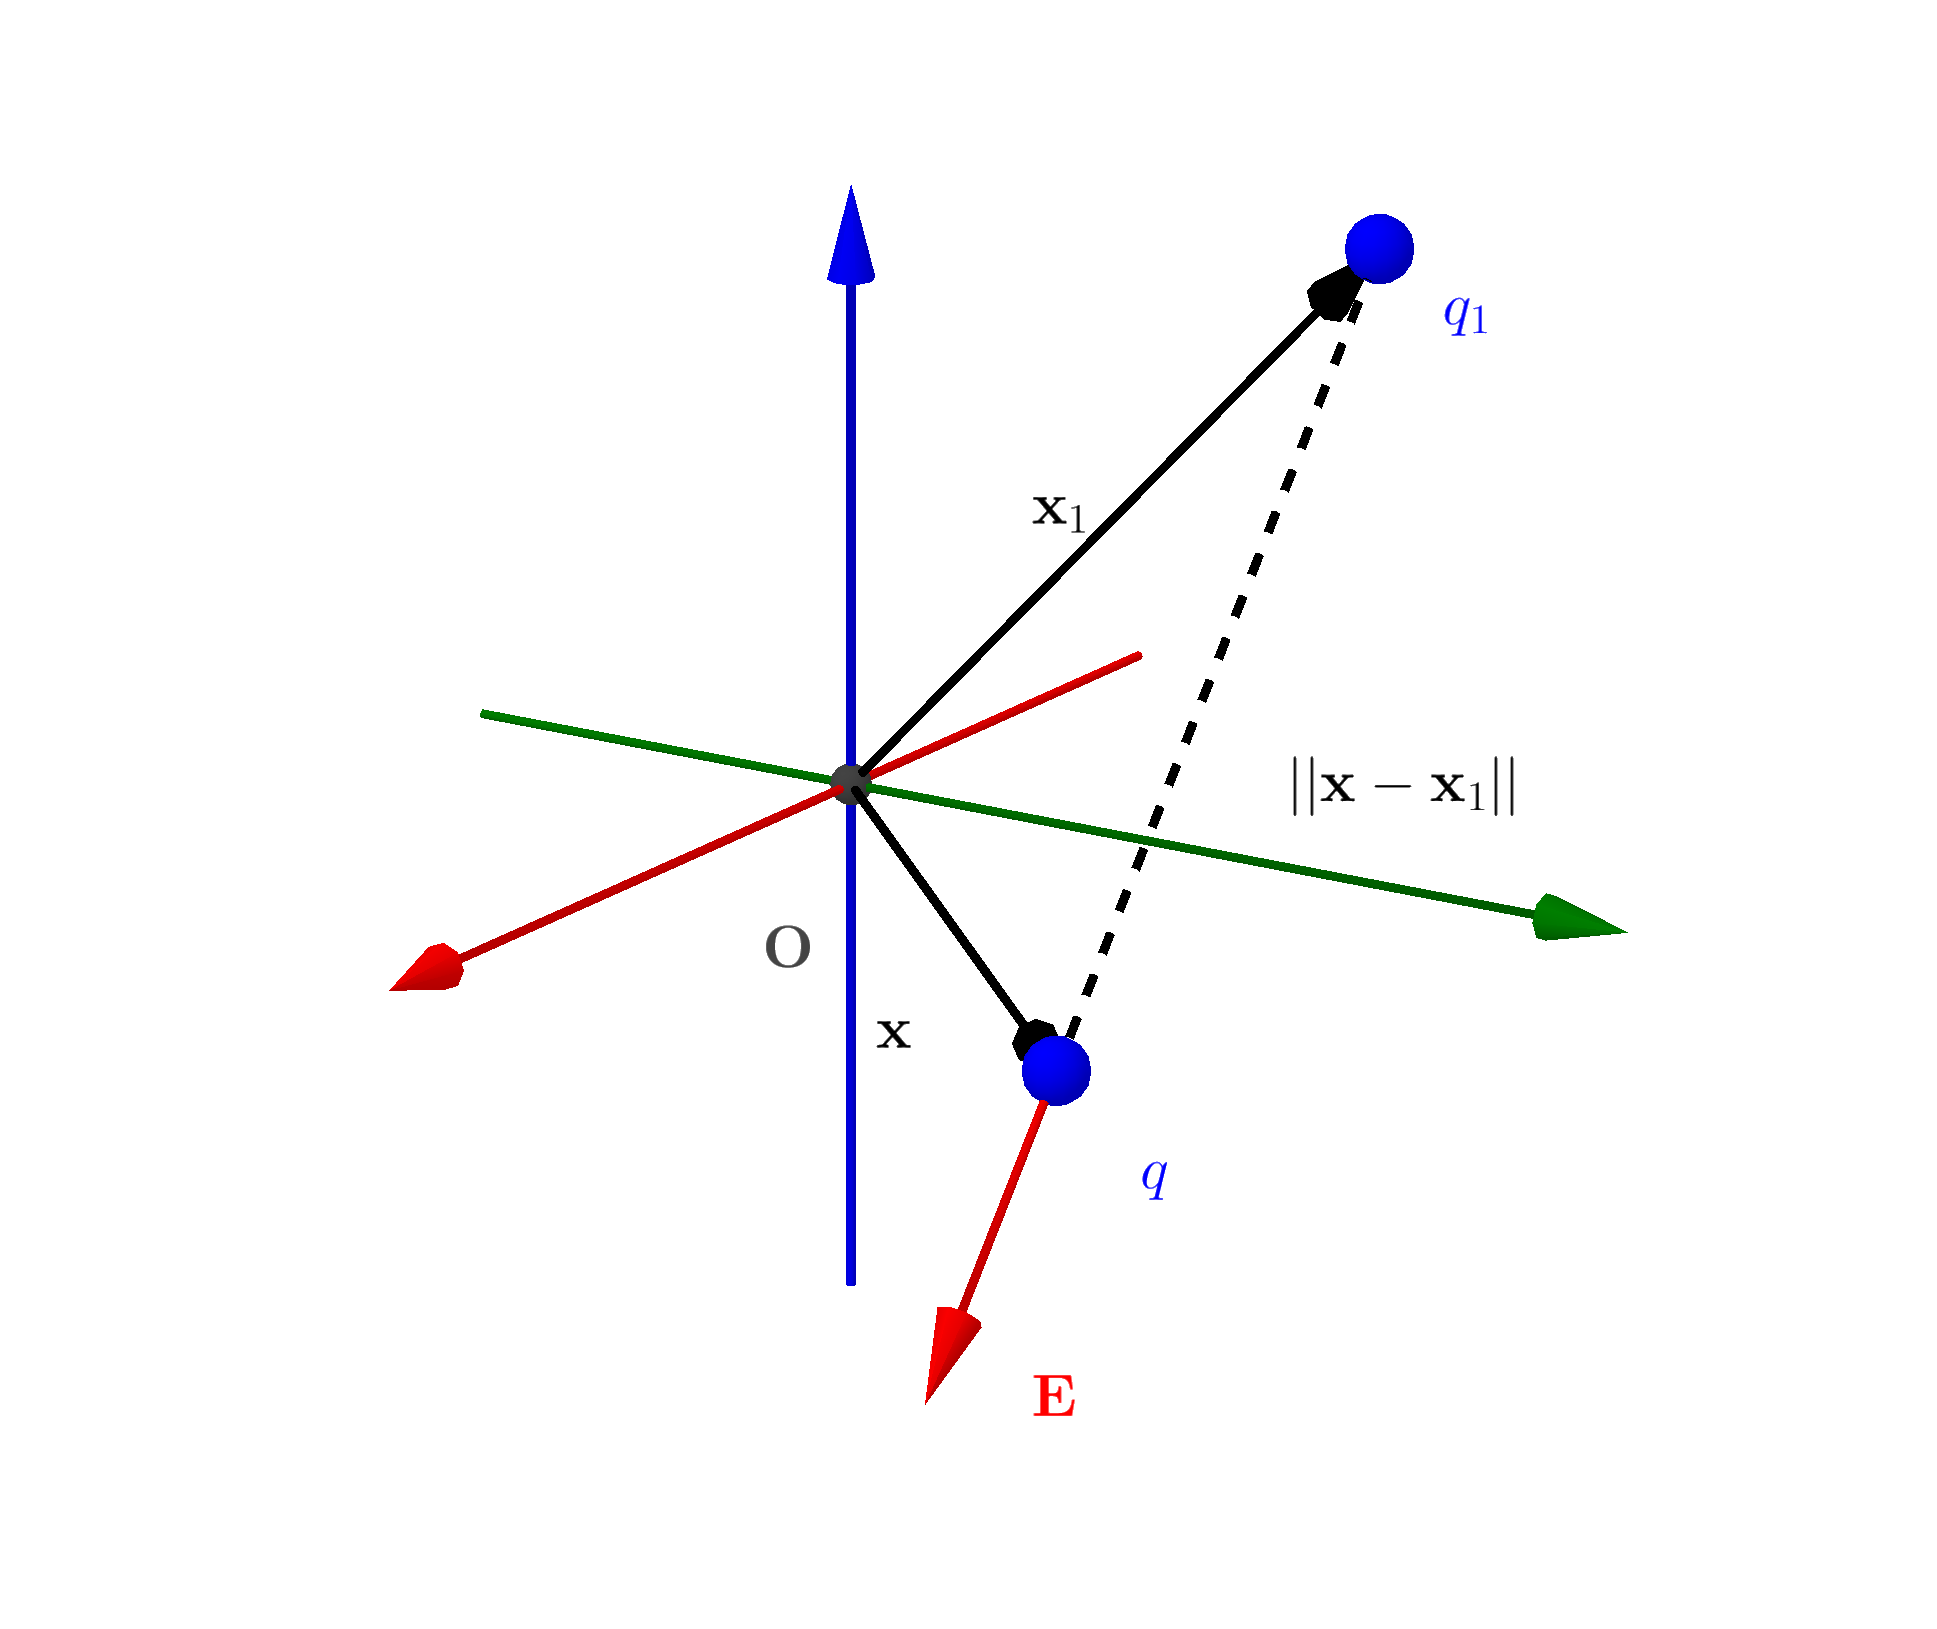
\includegraphics[scale=1]{camp_elet_3D}}
%\subfloat{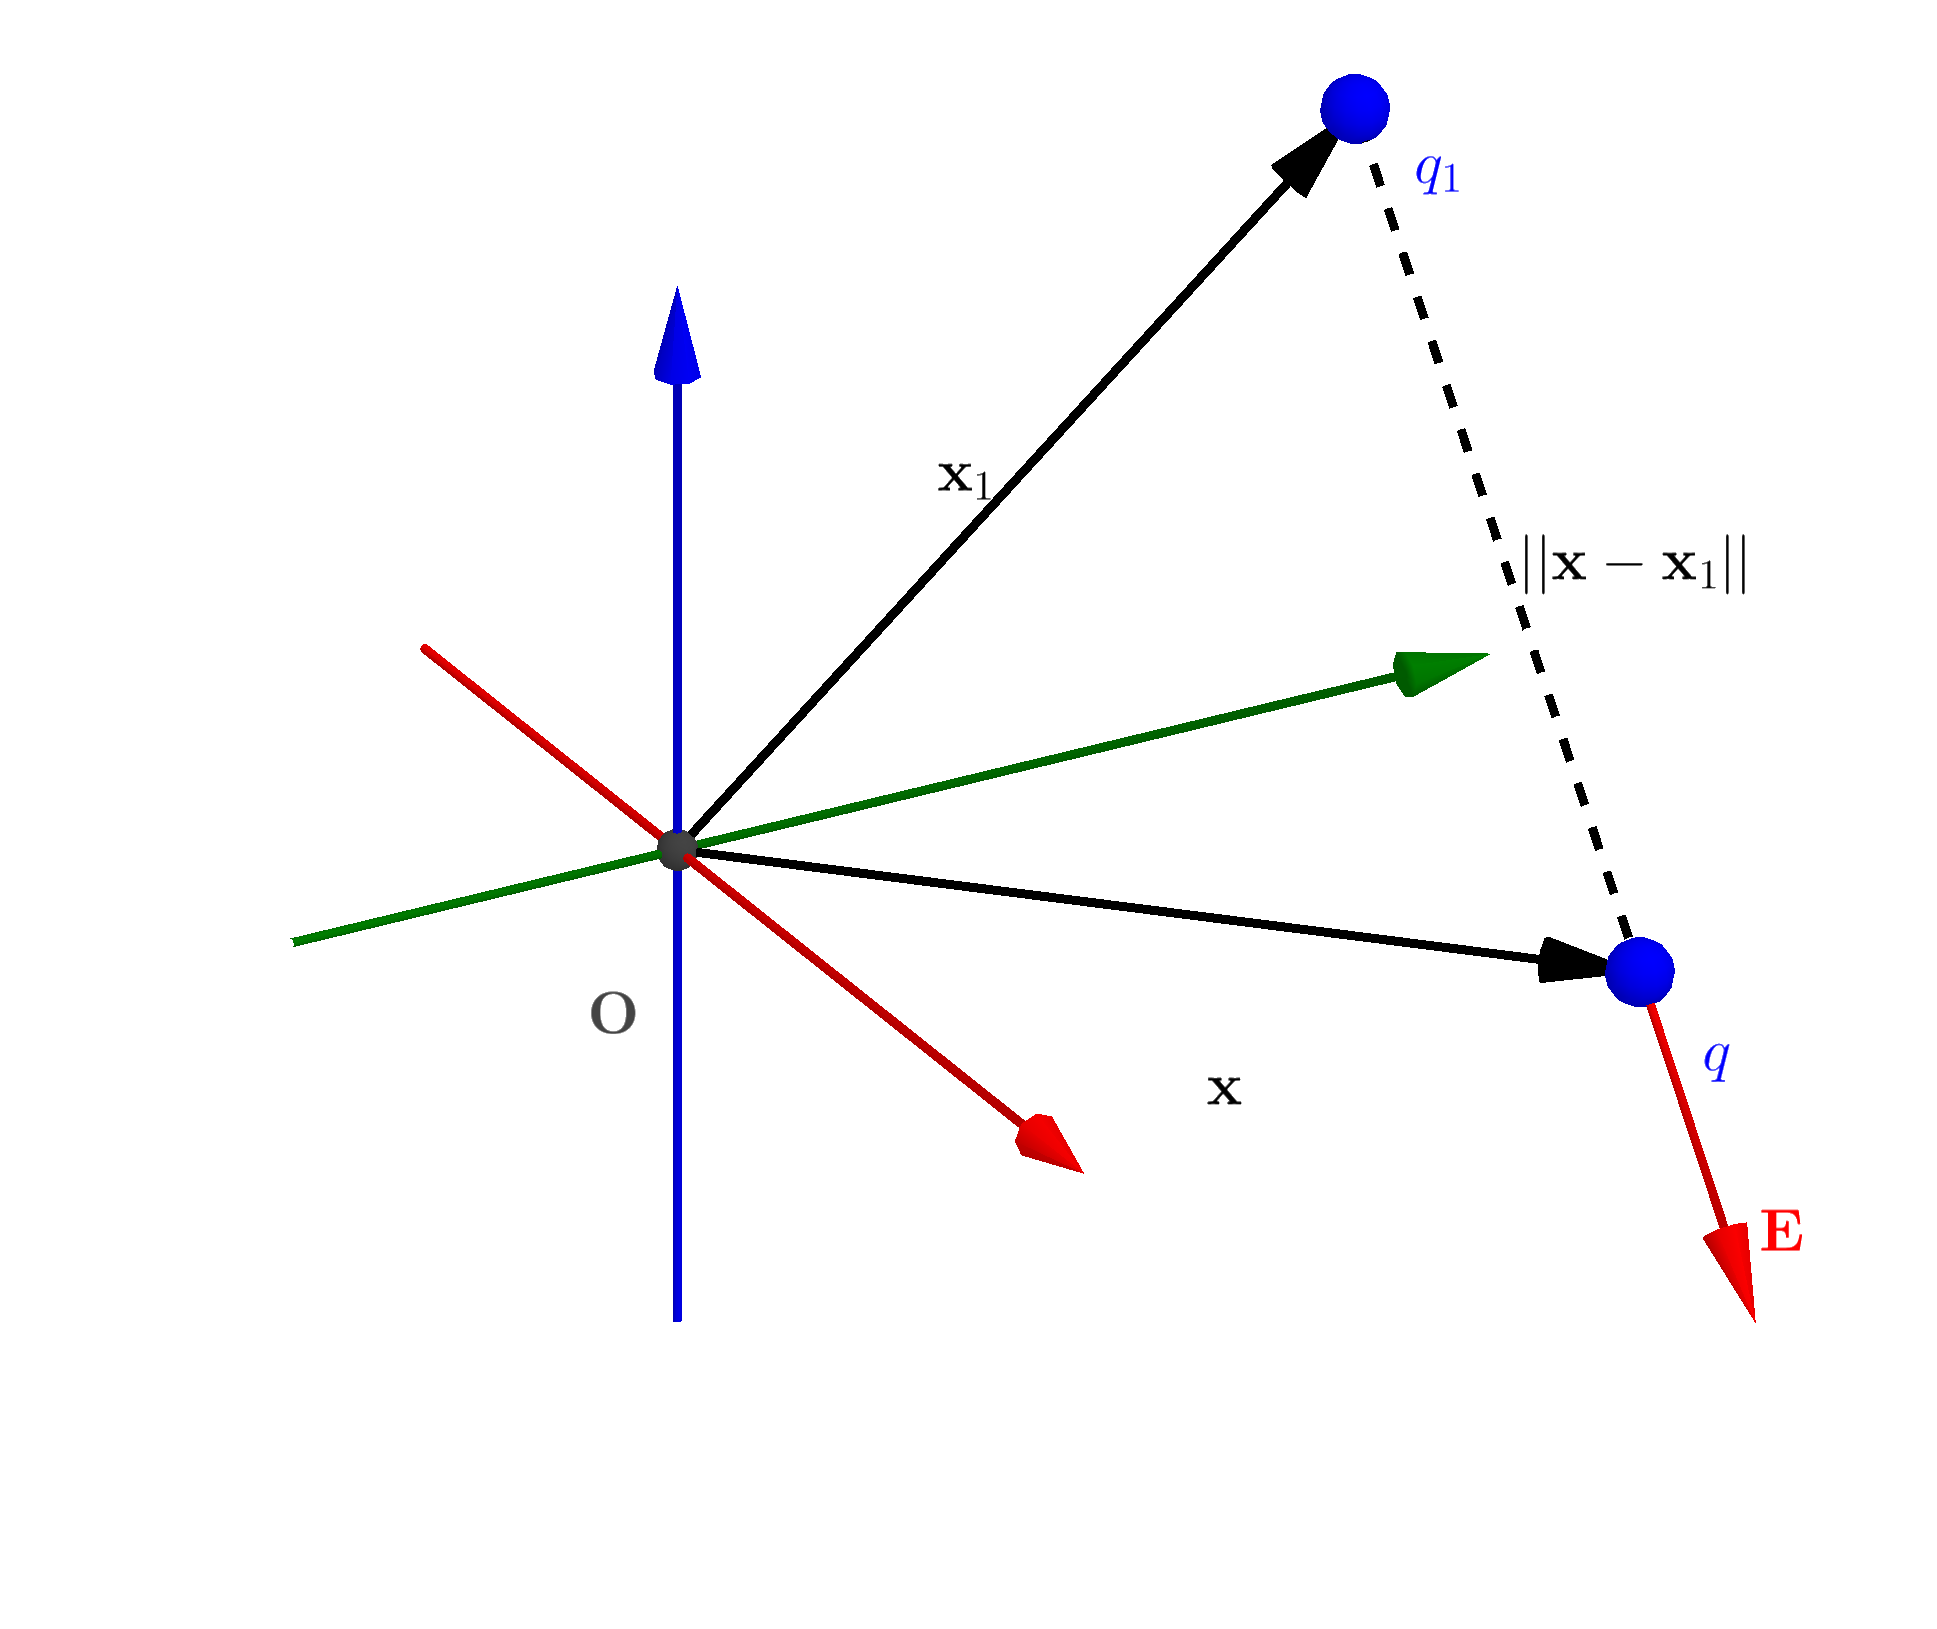
\includegraphics[scale=1]{camp_elet_3D2}}
%\caption{}
%\label{fig.mossul}
%\end{figure}

Num sistema com mais de uma carga fonte produzindo campos elétricos, foi observado experimentalmente que o campo elétrico total atuando num ponto $\textbf{x}$ é simplesmente o somatório dos campos produzidos por cada carga, o que ficou conhecido como a \textit{Superposição Linear} e pode ser expressada na forma
\begin{equation*}
\textbf{E}=k\,\sum_{i=1}^{n}q_i\,\frac{\textbf{x}_i-\textbf{x}}{||\textbf{x}_i-\textbf{x}||^3}.
\end{equation*} 
O campo elétrico devido a um pequeno número de cargas pode ser calculado a partir do princípio da superposição linear. Mas se temos uma quantidade muito grande de cargas num determinado volume $V$, devemos calcular a \textit{densidade volumétrica de carga elétrica} $\rho$ num volume infinitesimal situado em $\textbf{x}_0$ e em seguida integrar sobre o volume $V$ para obter a quantidade total de carga $Q$. A densidade de carga é definida por
\begin{equation*}
\rho(\textbf{x}_0)=\lim_{\Delta V_i \to 0}\frac{\Delta q_i}{\Delta V_i}=\frac{d\,q}{d\,V},
\end{equation*}
medida, no SI, em $C/m^3$. A quantidade total de carga $Q=\sum_i \Delta\,q_i$ no volume $V$ é
\begin{equation}\label{eq.densidade_carga}
Q=\int\int\int_{V}\rho(\textbf{x}_0)\,dV.
\end{equation}

O \textit{fluxo elétrico} é definido como a quantidade linhas do campo elétrico que atravessam uma superfície qualquer, e é dado pela equação
\begin{equation*}
\Phi_\textbf{E}=\textbf{E}\cdot\textbf{A}. 
\end{equation*} 
O \textit{vetor área} é definido como a magnitude da área da superfície atravessada apontando na direção do vetor normal à superfície, $\textbf{A}=A\,\textbf{n}$, e estamos considerando um campo elétrico uniforme $\textbf{E}$ que se desloca na direção $\textbf{n}$, ou seja, é perpendicular à superfície $A$ como podemos observar na figura \ref{fig.flux_ele}.
\begin{figure}[!htb]
\centering
\subfloat{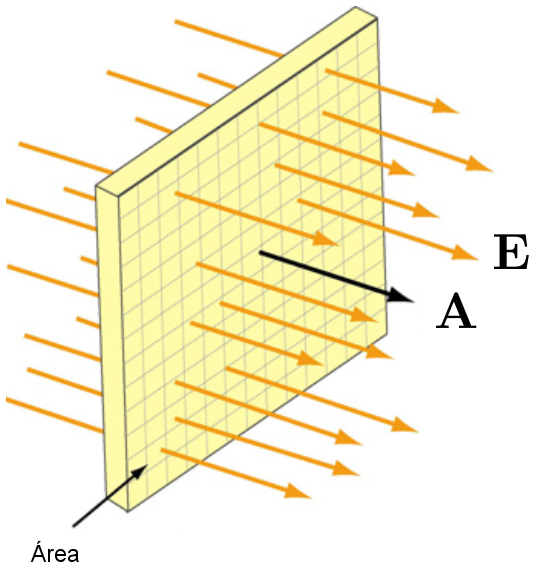
\includegraphics[scale=.4]{campo_area_2}}
\quad
\subfloat{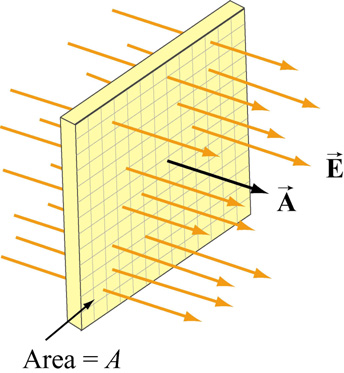
\includegraphics[scale=.4]{campo_area}}
\caption{\textit{Fluxo elétrico, linhas de campo elétrico passando através de uma superfície.}}
\label{fig.flux_ele}
\end{figure}
Mas se o campo elétrico se propaga formando um ângulo $\theta$ com o vetor normal da superfície, então o fluxo elétrico é dado por
\begin{equation*}
\Phi_\textbf{E}=\textbf{E}\cdot\textbf{A}=E\,A\,\cos\theta,
\end{equation*}
com $E=\textbf{E}\cdot\textbf{n}$ sendo a componente do campo elétrico na direção $\textbf{n}$. Em geral uma superfície $S$ pode ser curva e estamos interessados numa superfície \textit{fechada}, ou seja, aquela que engloba um determinado volume, o qual contém uma carga elétrica (exemplo na figura \ref{fig.esfe_gauss}). Tomando uma área bem pequena dessa superfície, $\Delta\textbf{A}_i$, o campo elétrico pode ser variável em cada parte da superfície e nessas condições temos que o fluxo nessa pequena região é dado por
\begin{equation*}
\Delta\,\Phi_\textbf{E}=\textbf{E}_i\cdot\Delta\,\textbf{A}_i.
\end{equation*}
O fluxo positivo atravessando toda a superfície de dentro para fora é calculado tomando o limite quando $\Delta\textbf{A}_i\to 0$ e aumentando infinitamente a quantidade dessas pequenas áreas até cobrir a superfície $S$
\begin{equation}\label{eq.fluxo_eletr}
\Phi_\textbf{E}=\lim_{i\to\infty}\sum_i\textbf{E}_i\cdot\textit{d}\textbf{A}_i=\int\int_S\textbf{E}\cdot\textit{d}\textbf{A}.
\end{equation}

Considere uma carga pontual positiva $q$ localizada no centro de uma esfera imaginária de raio $r$, onde essa carga produz um campo elétrico que aponta na direção radial conforme a figura \ref{fig.esfe_gauss}. Sabemos que a área da superfície dessa esfera é dada por $A=4\pi\,r^2$ e que, segundo a equação \ref{eq.campo_eletrico}, a magnitude do campo elétrico em qualquer ponto da superfície esférica é
\begin{equation*}
E=\frac{q}{4\pi\epsilon_0\,r^2},
\end{equation*}
assim o fluxo elétrico é calculado usando a equação \ref{eq.fluxo_eletr}.
\begin{align*}
\Phi_\textbf{E}&=\int\int_S\textbf{E}\cdot\textit{d}\textbf{A}\\
&=\int\int_S\textbf{E}\cdot\textbf{n}\,\textit{d}A\\
&=E\,\int\int_S\textit{d}A\\
&=E\,A\\
&=\frac{q}{4\pi\epsilon_0\,r^2}\,4\pi\,r^2\\
&=\frac{q}{\epsilon_0}.
\end{align*}
Na demonstração acima escolhemos uma esfera como \textit{superfície Gaussiana} mas, introduzindo o conceito de \textit{ângulo sólido}, vemos que a demonstração é válida para qualquer superfície fechada, utilizada em aplicações que apresentem mais ou menos alguma simetria (esférica, planar ou cilíndrica). Para mais detalhes consultar \cite{jackson_classical_1999}. Assim, concluímos que o fluxo elétrico através de uma superfície fechada que apresente mais ou menos alguma simetria é diretamente proporcional à quantidade de carga enclausurada pela superfície. Matematicamente, a \textit{lei de Gauss} para o fluxo elétrico é
\begin{equation}\label{eq.fluxo_eletrico}
\Phi_\textbf{E}=\int\int_S\textbf{E}\cdot\textit{d}\textbf{A}=\frac{q}{\epsilon_0}.
\end{equation}
\begin{figure}[!htb]
\centering
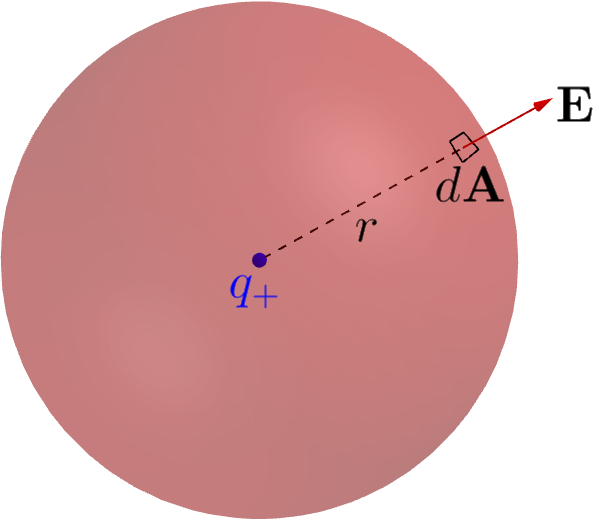
\includegraphics[scale=.3]{esfera_gaussiana}
\caption{\textit{Esfera Gaussiana enclausurando uma carga positiva $q$. Nessas condições, o ângulo entre o vetor campo elétrico e o vetor normal à superfície infinitesimal $d\textbf{A}$ é zero.}}
\label{fig.esfe_gauss}
\end{figure}

Uma carga elétrica produz um campo elétrico, e de maneira similar uma barra magnética, ou ímã, produz um \textit{campo magnético} $\textbf{B}$. Um ímã possui um polo norte de onde partem as linhas de campo magnético e um polo sul por onde as linhas de campo magnético retornam ao ímã (figura \ref{fig.barras_mag}). Diferentemente das cargas elétricas que são observadas isoldamente na natureza, os dois polos magnéticos sempre aparecem aos pares, ou seja, monopolos magnéticos não existem isoladamente apesar de a suposição de sua existência ser de interesse teórico. Assim, sempre que um ímã é fracionado, mesmo que em partes muito elementares, o resultado sempre será um novo ímã com dois polos magnéticos conforme a figura \ref{fig.barras_mag}.
\begin{figure}[!htb]
\centering
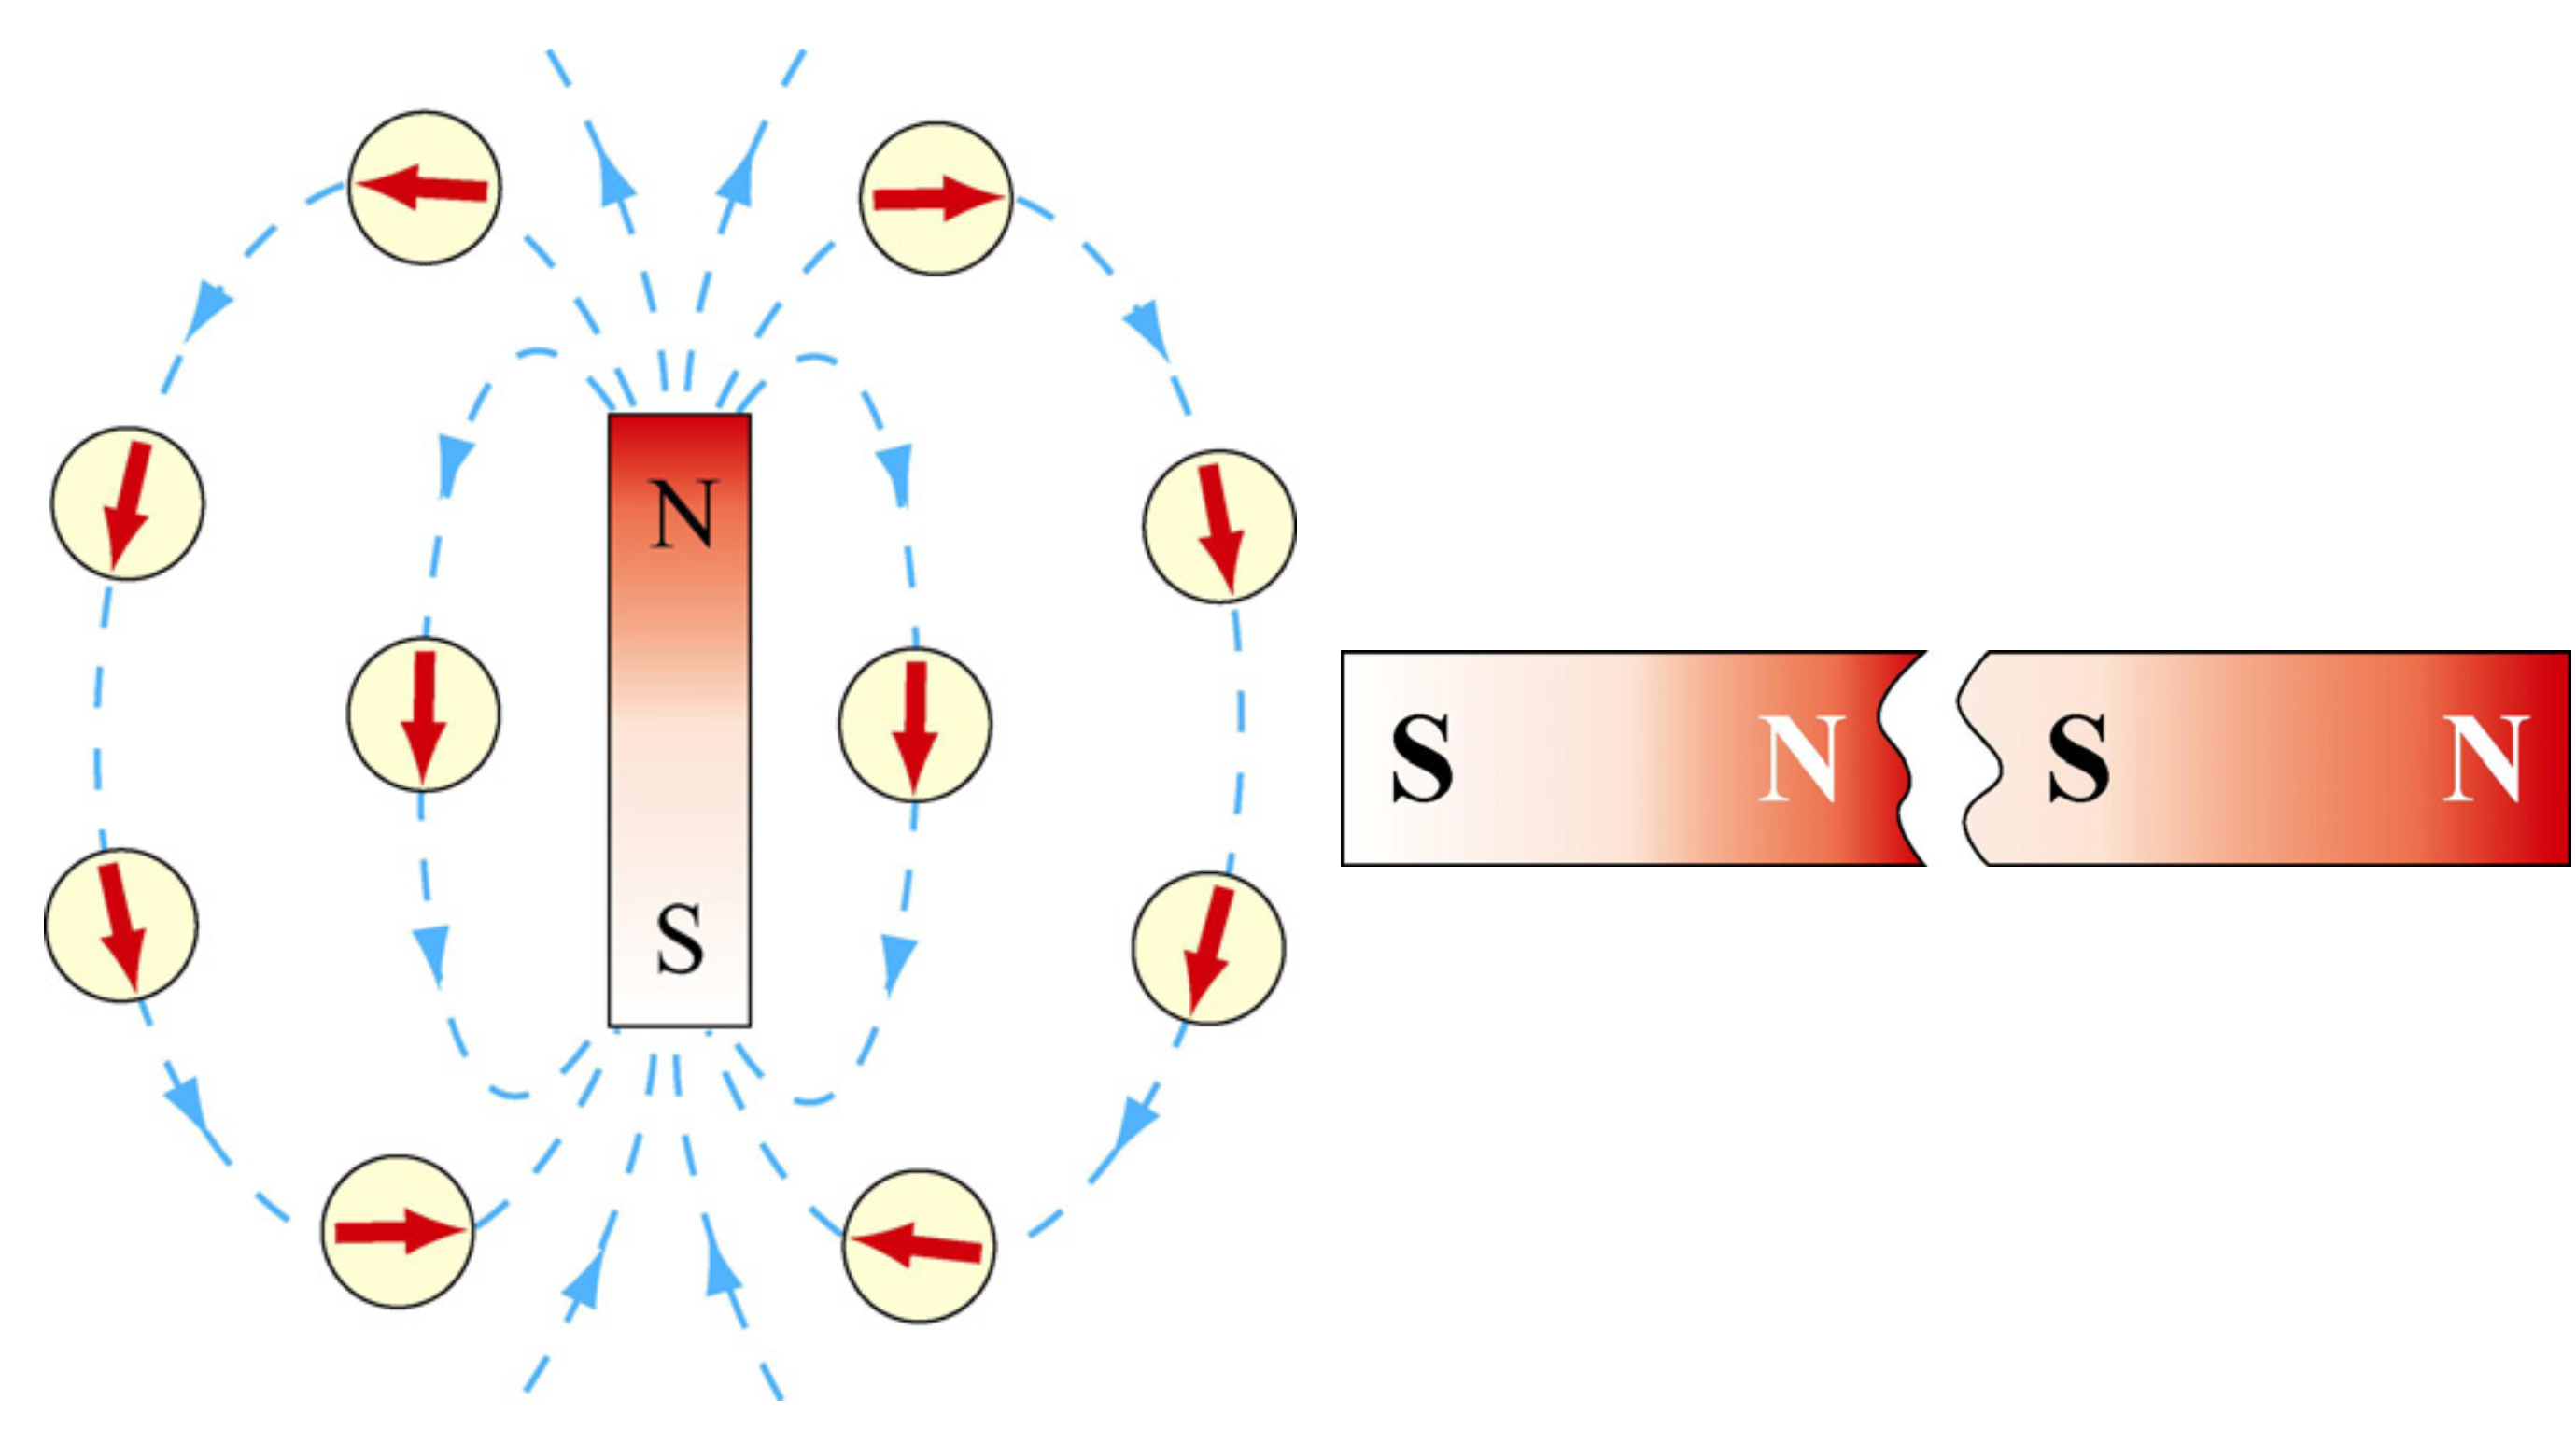
\includegraphics[scale=.7]{barras_magn}
\caption{\textit{Barras magnéticas onde polos de mesmo sinal se repelem e polos de sinais contrários se atraem.}}
\label{fig.barras_mag}
\end{figure}
Como não existem monopolos magnéticos, o campo magnético deve ser definido de forma diferente do campo elétrico, e experimentalmente foram observadas algumas características relacionadas ao movimento de uma carga elétrica $q$ com velocidade $\textbf{v}$ num campo magnético $\textbf{B}$:
\begin{itemize}
\item a magnitude da força magnética $\textbf{F}_B$ é proporcional à $v$, $B$ e $q$, onde $v$ e $B$ são as magnitudes da velocidade e do campo magnético respectivamente,
\item a direção de $\textbf{F}_B$ é perpendicular ao plano formado por $\textbf{v}$ e $\textbf{B}$,
\item $\textbf{F}_B$ é proporcional ao $\sin\theta$, o ângulo formado por $\textbf{v}$ e $\textbf{B}$. Se $\textbf{v}$ e $\textbf{B}$ são paralelos então $\textbf{F}_B=0$, e
\item o sentido de $\textbf{F}_B$ depende do sinal da carga $q$.
\end{itemize}
Essas observações são ilustradas na figura \ref{fig.froca_mag_veloc} e a força magnética é definida como
\begin{equation*}
\textbf{F}_B=q\,\textbf{v}\times\textbf{B}.
\end{equation*}
\begin{figure}[!htb]
\centering
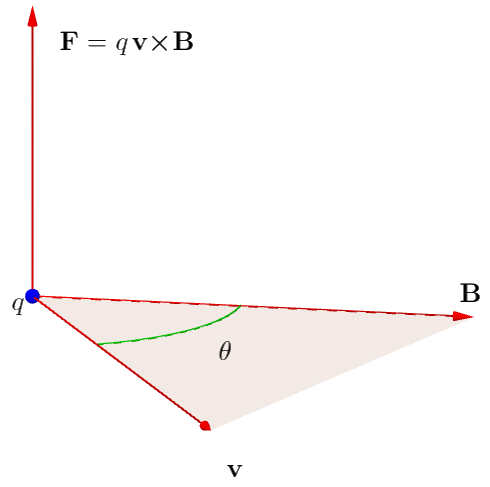
\includegraphics[scale=.4]{forca_camp_mag_veloc}
\caption{\textit{Força magnética agindo numa carga elétrica que se desloca num campo magnético.}}
\label{fig.froca_mag_veloc}
\end{figure}
Teoricamente, poderíamos tentar determinar a lei de Gauss para o fluxo magnético com o mesmo procedimento aplicado ao fluxo elétrico e obter
\begin{equation*}
\Phi_\textbf{B}=\int\int_S\textbf{B}\cdot\textit{d}\textbf{A}=\frac{q_m}{\mu_0},
\end{equation*} 
onde $q_m$ é a carga magnética (suposto monopolo magnético) enclausurado pela superfície Gaussiana, $\mathbf{B}$ é o campo magnético e $\mu_0$ é a \textit{permeabilidade magnética no vácuo} com valor $\mu_0=4\,\pi\times 10^{-7}\, T\,m/A$. No entanto, não foi constatada a existência de qualquer carga magnética isolada mesmo após muitos esforços. Como $q_m=0$, temos que a lei de Gauss para o magnetismo é
\begin{equation}\label{eq.gauss_flux_mag}
\Phi_\textbf{B}=\int\int_S\textbf{B}\cdot\textit{d}\textbf{A}=0.
\end{equation}
Conforme podemos ver na figura \ref{fig.flux_elet_magn}, a equação \ref{eq.gauss_flux_mag} implica que a quantidade de linhas do campo magnético saindo da superfície é igual à quantidade que está entrando, ou seja, não há uma origem isolada e um término isolado para o fluxo magnético como há para o fluxo elétrico. Outro problema é que a barra imantada atravessa a superfície que, de acordo com a hipóteses da lei de Gauss, deveria ser fechada.
\begin{figure}[!htb]
\centering
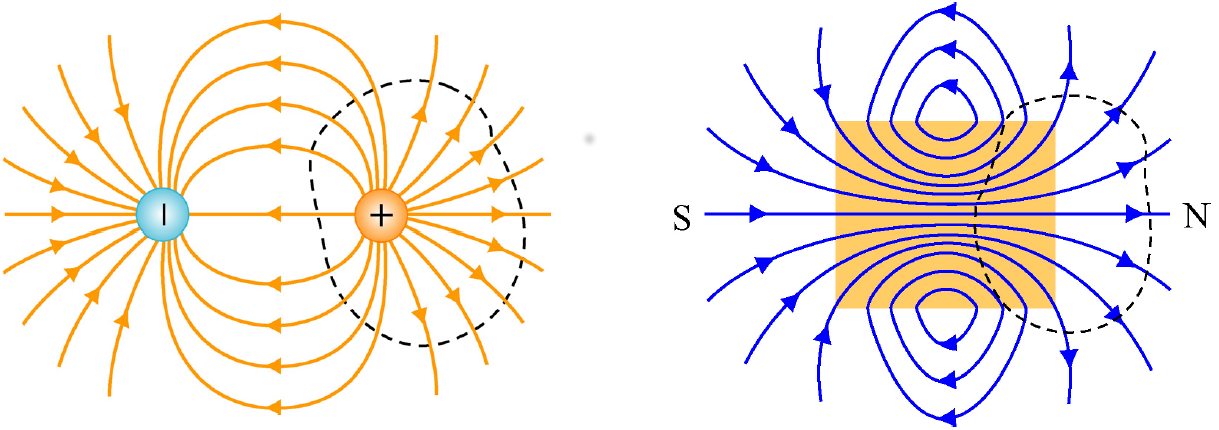
\includegraphics[scale=.3]{flux_ele_mag}
\caption{\textit{As linhas do campo magnético que emanam do polo norte do ímã em direção ao polo sul retornam para dentro da superfície Gaussiana descrevendo um laço fechado.}}
\label{fig.flux_elet_magn}
\end{figure}

\subsection{A Lei de Ampère}
Correntes elétricas podem ser produzidas por cargas elétricas que se movem num fio condutor. Essas correntes elétricas são fontes de campos magnéticos $d\,\textbf{B}$, num determinado ponto $\mathbf{x}$, e que podem ser calculados em função da corrente $I$ num intervalo infinitesimal $d\,\textbf{l}$ do fio. Visualização na figura \ref{fig.corrente_fio}. A fonte de corrente infinitesimal é dada por $I\,d\,\textbf{l}$ e $r$ é a distância entre o ponto de aplicação do campo magnético e a fonte de corrente infinitesimal. O vetor $\textbf{n}$ é o vetor normal que aponta na direção de $\mathbf{x}$ e o vetor $d\,\textbf{l}$ aponta na direção e sentido da corrente $I$. Repare ainda que o campo magnético depende do ângulo $\theta$ entre $\mathbf{n}$ e $d\mathbf{l}$.
\begin{figure}
\centering
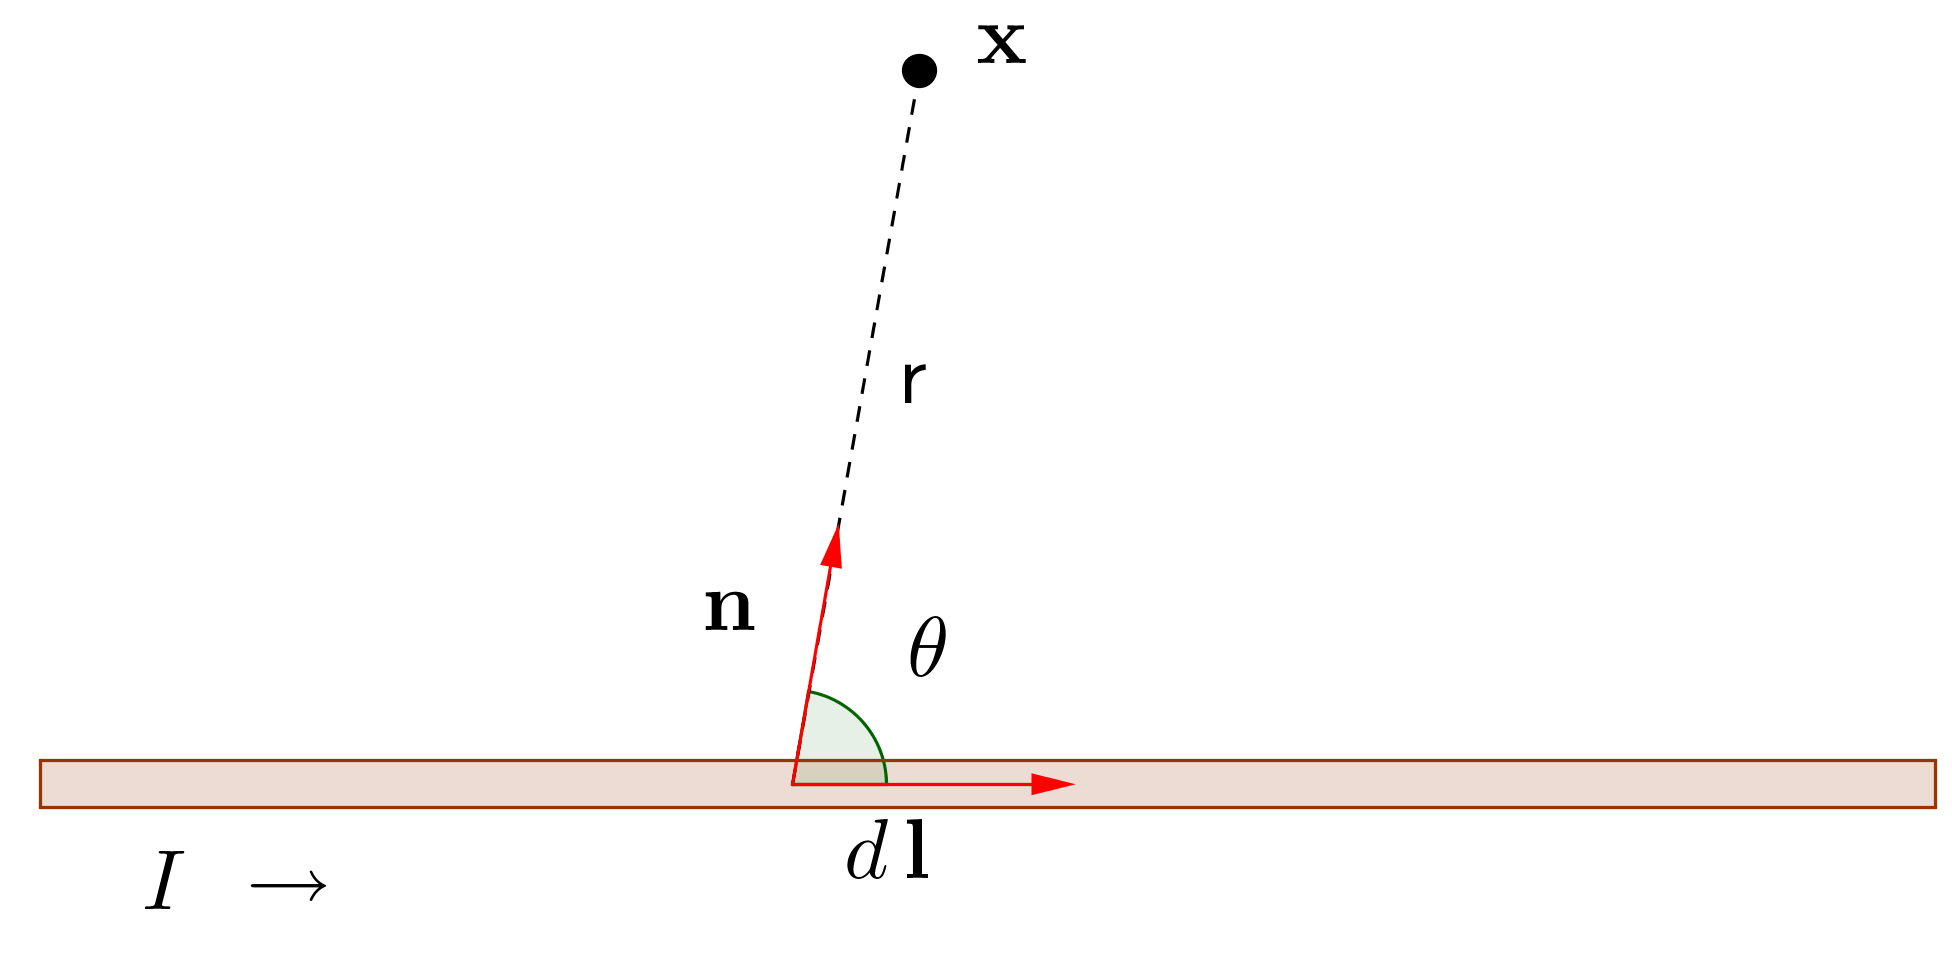
\includegraphics[scale=1.1]{corrente_fio}
\caption{\textit{Campo magnético no ponto $\mathbf{x}$ devido a passagem de uma corrente elétrica $I$ pelo fio. Observe que a magnitude do campo depende também do ângulo $\theta$ entre $\textbf{l}$ e $\textbf{n}$}.}
\label{fig.corrente_fio}
\end{figure}
Assim sendo, a \textit{Lei de Biot-Savart} tem definição análoga à do campo elétrico (derivada da lei de Coulomb) e pode ser expressa como
\begin{equation}\label{eq.lei_biot_savart}
d\,\textbf{B}=\frac{\mu_0}{4\,\pi}\frac{I}{r^2}\,d(\textbf{l}\times\textbf{n}),
\end{equation}
e o campo magnético no volume ao redor do fio pode ser obtido integrando sobre a direção perpendicular ao plano formado por $\textbf{l}$ e $\textbf{n}$ ao longo do comprimento do fio.
\begin{equation}
\textbf{B}=\frac{\mu_0I}{4\,\pi}\int_{\textbf{l}}\frac{d(\textbf{l}\times\textbf{n})}{r^2}.
\end{equation}

Considere agora um laço circular (linha de campo magnético) de raio $r$ contido num plano perpendicular ao fio condutor, onde esse laço está dividido em pequenos comprimentos $\Delta\textbf{s}=\Delta s\,\pmb{\phi}$, cujos vetores correspondentes a cada ponto do laço apontam na direção do vetor tangencial à circunferência naquele ponto, conforme  a figura \ref{fig.laco_amperiano}. Esse laço fechado contido num plano é denominado \textit{laço Amperiano} e é usado para calcular o campo magnético referente àquela linha de campo tomando o limite quando $\Delta\textbf{s}\to 0$ e integrando no intervalo dado pelo comprimento da circunferência. Nesse caso, $\theta=\pi$ e $\pmb{\phi}$ é perpendicular ao plano formado por $\textbf{l}$ e $\textbf{n}$, portanto a magnitute do vetor  $\textbf{B}$ na direção $\pmb{\phi}$ é dada pela lei de Biot-Savart na equação \ref{eq.lei_biot_savart}.
\begin{equation*}
\int_{s}\textbf{B}\cdot d\textbf{s}=B\int_{s}ds=\frac{\mu_0I}{2\pi\,r}2\pi\,r=\mu_0I.
\end{equation*} 
\begin{figure}[h]
\centering
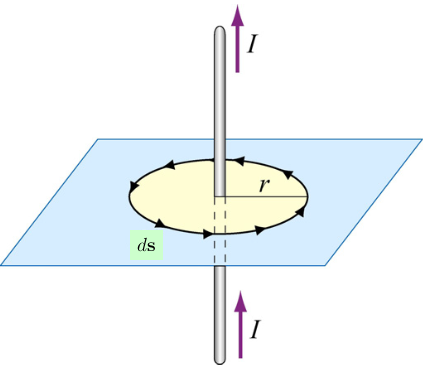
\includegraphics[scale=.5]{laco_amperiano}
\caption{\textit{Laço amperiano seguindo a regra da mão direita: posicionando o polegar no sentido da corrente, o campo magnético tem o mesmo sentido dos demais dedos curvando em torno do fio.}}
\label{fig.laco_amperiano}
\end{figure}

Vamos considerar um outro exemplo de laço amperiano cujo contorno denotado por $abcda$ se sobrepõe a duas linhas de campo magnético coplanares, observado na figura \ref{fig.laco_amper_2}. No desenvolvimento abaixo, a primeira e terceira integrais zeram pois o campo magnético é perpendicular ao caminho de integração nesses intervalos, e $B_2(r_2\theta)$ e $B_1[r_1(2\pi-\theta)]$ são os comprimentos dos arcos $bc$ e $da$, respectivamente. A integral de linha do campo magnético no contorno $abcda$ é
\begin{align*}
\int_{abcda}\textbf{B}\cdot d\textbf{s}&=\int_{ab}\textbf{B}\cdot d\textbf{s}+\int_{bc}\textbf{B}\cdot d\textbf{s}+\int_{cd}\textbf{B}\cdot d\textbf{s}+\int_{da}\textbf{B}\cdot d\textbf{s}\\
&=0+B_2(r_2\theta)+0+B_1[r_1(2\pi-\theta)]\\
&=\frac{\mu_0I}{2\pi\,r_2}(r_2\theta)+\frac{\mu_0I}{2\pi\,r_1}[r_1(2\pi-\theta)]\\
&=\frac{\mu_0I}{2\pi}\theta+\frac{\mu_0I}{2\pi}(2\pi-\theta)\\
&=\mu_0I.
\end{align*}
\begin{figure}
\centering
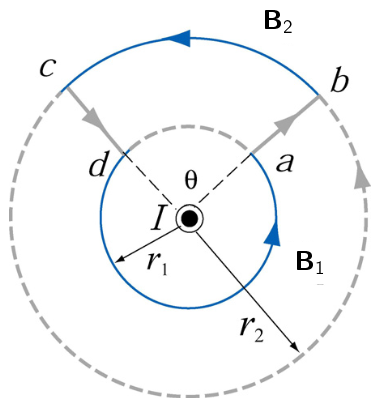
\includegraphics[scale=.5]{laco_amperiano_2}
\caption{\textit{Laço amperiano passando por duas linhas de campo magnético. O ponto no centro significa que o sentido da corrente elétrica está ``saindo do plano do papel".}}
\label{fig.laco_amper_2}
\end{figure}
Vemos o mesmo resultado se o laço amperiano envolve uma ou duas linhas de campo magnético e, usando coordenadas cilíndricas, podemos demonstrar que o mesmo resultado é válido para uma quantidade arbitrária de linhas de campo magnético, ou seja, a integral de linha do campo magnético através de qualquer laço amperiano fechado é proporcional à corrente elétrica inscrita no laço. A \textit{Lei de Ampère} é dada por
\begin{equation*}
\int_{s}\textbf{B}\cdot d\textbf{s}=\mu_0I.
\end{equation*}
Analogamente à lei de Gauss para campos elétricos, para ser aplicada a lei de Ampère é necessário que o laço possua alguma simetria em relação ao fio. No caso de um fio condutor suficientemente comprido para que suas extremidades não interfiram na aplicação, temos uma simetria cilíndrica e a lei de Ampère pode ser aplicada normalmente. Caso o fio não seja suficientemente comprido, devemos utilizar a lei de Biot-Savart. 

Agora considere a seguinte situação, descrita por Maxwell, onde o circuito elétrico está interrompido por um capacitor. 
\begin{figure}
\centering
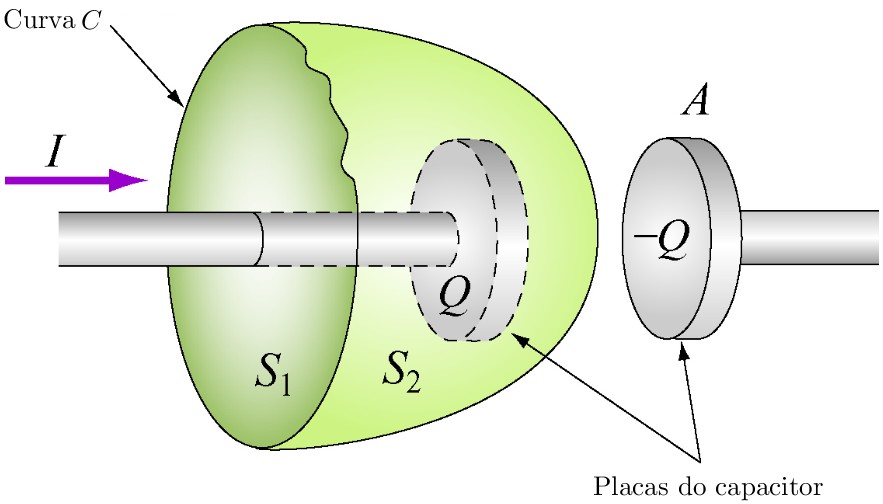
\includegraphics[scale=.3]{capacitor}
\caption{\textit{Quando há corrente no circuito, cargas positivas se acumulam numa placa do capacitor assim como cargas negativas se acumulam na outra placa. Tal acúmulo gera um fluxo elétrico variável entre as placas.}}
\label{fig.capacitor}
\end{figure}
Como vimos pela lei de Ampère, o campo magnético depende somente da corrente no circuito e do comprimento da circunferência que limita a superfície atravessada pelo fio condutor, e não depende dessa superfície em si. Portanto, o campo magnético referente à curva $C$ da figura \ref{fig.capacitor} pode ser calculado considerando a superfície $S_1$ ou a superfície $S_2$. A superfície $S_1$ é atravessada pela corrente $I$ a qual produz o campo magnético $\mathbf{B}$, mas superfície $S_2$ não é atravessada por $I$ e, no entanto, é produzido o mesmo campo magnético $\mathbf{B}$. Assim podemos sugerir que exista um outro fenômeno físico entre as placas do capacitor que seja responsável pela geração de $\mathbf{B}$. À medida que o capacitor vai sendo carregado, cargas elétricas opostas vão se acumulando em suas placas gerando um campo elétrico variável entre as placas, o qual produz um fluxo elétrico variável através da área da placa do capacitor. Maxwell mostrou que o produto da variação desse fluxo elétrico pela permissividade elétrica no vácuo era numericamente igual à corrente $I$, e por isso produzia o mesmo campo $\mathbf{B}$ quando integrado longo da curva $C$,
\begin{equation*}
I_d=\epsilon_0\frac{d\phi_E}{dt}.
\end{equation*}
Tal produto foi denominado \textit{corrente deslocada} e foi adicionado à lei de Ampère, a qual se tornou a \textit{lei de Ampére generalizada} ou \textit{lei de Ampère-Maxwell},
\begin{equation}\label{eq.ampere_generalizada}
\int_s\mathbf{B}\cdot d\mathbf{s}=\mu_0I+\mu_0\epsilon_0\frac{d\phi_E}{dt}.
\end{equation}
Note que quando consideramos a superfície $S_1$, $I_d=0$ já que o fluxo elétrico é constante e assim $\mathbf{B}$ é dado somente por $I$. Quando consideramos a superfície $S_2$, $I=0$ e $\mathbf{B}$ é dado somente por $I_d$. 




\subsection{A Lei de Faraday}
Analogamente ao caso da força gravitacional, o \textit{trabalho} $W$ realizado por uma força elétrica $\textbf{F}_e$ para levar uma carga elétrica $q$ de um ponto $A$ até um ponto $B$ é definido como
\begin{equation}\label{eq.trabalho}
W=\int_{A}^{B}\textbf{F}_e\cdot d\textbf{s}.
\end{equation}
A diferença entre a \textit{energia potencial} $U$ em cada um dos pontos $A$ e $B$ é o que ocasiona o deslocamento da carga, assim a variação da energia potencial tem definição
\begin{equation}\label{eq.energia_potencial}
\Delta U=U_b-U_a=-\int_{A}^{B}\textbf{F}_e\cdot d\textbf{s}=-W.
\end{equation}
A \textit{diferença de potencial elétrico}, $\Delta V$, também chamada \textit{ddp}, é a variação da energia potencial por unidade de carga elétrica $q$. Utilizando a equação \ref{eq.camp_elet}, que relaciona força elétrica e campo elétrico, podemos definir a ddp como
\begin{equation}\label{eq.ddp}
\Delta V=-\int_{A}^{B}\frac{\textbf{F}_e}{q}\cdot d\textbf{s}=-\int_{A}^{B}\textbf{E}\cdot d\textbf{s}
\end{equation}
A ddp representa a quantidade de trabalho por unidade de carga para mover a carga do ponto $A$ ao ponto $B$ e sua unidade de medida no SI é o volt ($V=\frac{J}{C}$). Observe nas definições acima que só importa os valores no pontos $A$ e $B$, e não importa necessariamente o caminho que a carga vai percorrer de um ponto até o outro. 

Agora, num circuito elétrico fechado, as cargas percorrem um determinado caminho a partir de uma fonte de energia elétrica. Essa fonte é chamada de \textit{força eletromotriz}, representada por $\varepsilon$, e que pode ser pensada como uma ``bomba" de cargas que as impulsiona de um potencial menor para um potencial maior. A força eletromotriz é definida como o trabalho realizado para mover uma carga unitária na direção de maior potencial, matematicamente,
\begin{equation*}
\varepsilon=\frac{dW}{dq}, 
\end{equation*}
também medida em volt. Como o campo magnético não produz trabalho, o trabalho realizado sobre o movimento das cargas deve ser devido a um campo elétrico e para escrever a força eletromotriz em termos do campo elétrico de forma análoga ao que foi feito nas equações \ref{eq.trabalho}, \ref{eq.energia_potencial} e \ref{eq.ddp}, devemos utilizar uma integral de linha, pois nesse caso a corrente percorre um determinado caminho. Como o campo elétrico é não-conservativo (senão não haveria corrente) o valor da integral na equação \ref{eq.ddp} é diferente de zero. Assim,
\begin{equation}\label{eq.emf_E_nc}
\varepsilon=\int_s\pmb{E}\cdot d\pmb{s}.
\end{equation}
 
O \textit{fluxo magnético} é definido de maneira similar ao fluxo elétrico e seu entendimento também pode ser acompanhado pela figura \ref{fig.flux_ele}. O fluxo magnético através de uma superfície é definido como
\begin{equation*}
\phi_\mathbf{B}=\textbf{B}\textbf{A}=B\,A\,\cos\theta,
\end{equation*}
onde o vetor área é $\textbf{A}=A\textbf{n}$, $\textbf{n}$ é o vetor normal à superfície atravessada, $A$ é a magnitude da área, $B=\textbf{B}\cdot\textbf{n}$ é a componente do campo magnético na direção do vetor normal e $\theta$ é o ângulo entre $\textbf{B}$ e $\pmb{A}$. Tomando um elemento infinitesimal da área e integrando sobre a superfície o fluxo magnético é
\begin{equation}\label{eq.fluxo_mag}
\phi_{\mathbf{B}}=\int\int_S\pmb{B}\,d\pmb{A},
\end{equation}
medido em \textit{Weber}, $T/m^2$. 

Em 1831, Faraday descobriu que se pode criar um campo elétrico variando um campo magnético em função do tempo num fenômeno que foi batizado de \textit{indução eletromagnética}. Um dos experimentos de Faraday (figura \ref{fig.exper_faraday}) consiste em movimentar um ímã dentro de uma bobina feita de fio condutor onde se pode observar a geração de uma corrente elétrica, como se a bobina estivesse conectada a fonte de força eletromotriz. O experimento mostra que a força eletromotriz induzida é proporcional à taxa (negativa) de variação do fluxo magnético através da bobina, a \textit{lei de Faraday} é
\begin{equation*}
\varepsilon=-\frac{d\phi_\mathbf{B}}{dt}.
\end{equation*}
Podemos reescrever a lei de Faraday usando a equação \ref{eq.emf_E_nc},
\begin{equation}\label{eq.lei_faraday}
\varepsilon=\int_s\pmb{E}\cdot d\pmb{s}=-\frac{d\phi_\mathbf{B}}{dt},
\end{equation}
o que implica que a variação do fluxo magnético induz um campo elétrico não-conservativo que varia com o tempo, diferente do campo elétrico conservativo gerado por cargas elétricas estacionárias.

\begin{figure}[!htb]
\centering
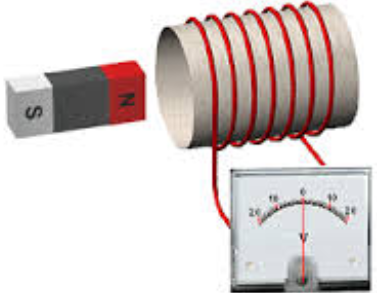
\includegraphics[scale=.5]{experi_faraday}
\caption{\textit{Experimento de indução eletromagnética promovido por Michael Faraday.}}
\label{fig.exper_faraday}
\end{figure}


\section{Equações de Maxwell}
Vimos pela equação \ref{eq.fluxo_eletrico}, que o fluxo elétrico através de uma superfície fechada é proporcional à quantidade de carga elétrica enclausurada por essa superfície. Quando temos uma quantidade de carga muito grande devemos calcular o fluxo elétrico devido à densidade carga, e substituindo a equação \ref{eq.densidade_carga} na equação \ref{eq.fluxo_eletrico} temos
\begin{align*}
\int\int_S\textbf{E}\cdot\textit{d}\textbf{A}&=\frac{q}{\epsilon_0}\\
&=\frac{Q}{\epsilon_0}\\
&=\frac{1}{\epsilon_0}\int\int\int_{V}\rho\,dV\\
\int\int_S\epsilon_0\textbf{E}\cdot\textit{d}\textbf{A}&=\int\int\int_{V}\rho\,dV.
\end{align*}
A equação acima é conhecida como a primeira equação de Maxwell para o eletromagnetismo escrita na forma integral. 


A segunda equação de Maxwell é similar à primeira e, como não existem monopolos magnéticos, tal equação fica definida como a propria equação \ref{eq.gauss_flux_mag} já discutida na subseção \ref{sec.lei_gauss},
\begin{equation*}
\int\int_S\textbf{B}\cdot\textit{d}\textbf{A}=0.
\end{equation*}


A \textit{corrente elétrica média} é definida como a taxa com que uma quantidade de carga atravessa uma determinada área de seção transversal de um meio condutor,
\begin{equation*}
I_m=\frac{\Delta\,Q}{\Delta\,t},
\end{equation*}
medida em coulomb por segundo $(C/s)$ no SI. Em termos microscópicos, a quantidade de carga que atravessa uma superfície num determinado tempo é dada em função da \textit{densidade de corrente elétrica} $\mathbf{J}$,
\begin{equation}\label{eq.densidade_corrente}
I=\int\int_S\mathbf{J}\cdot\,d\mathbf{A},
\end{equation}
onde a densidade de corrente elétrica é medida em $(A/m^2)$ no SI. 
\begin{figure}
\centering
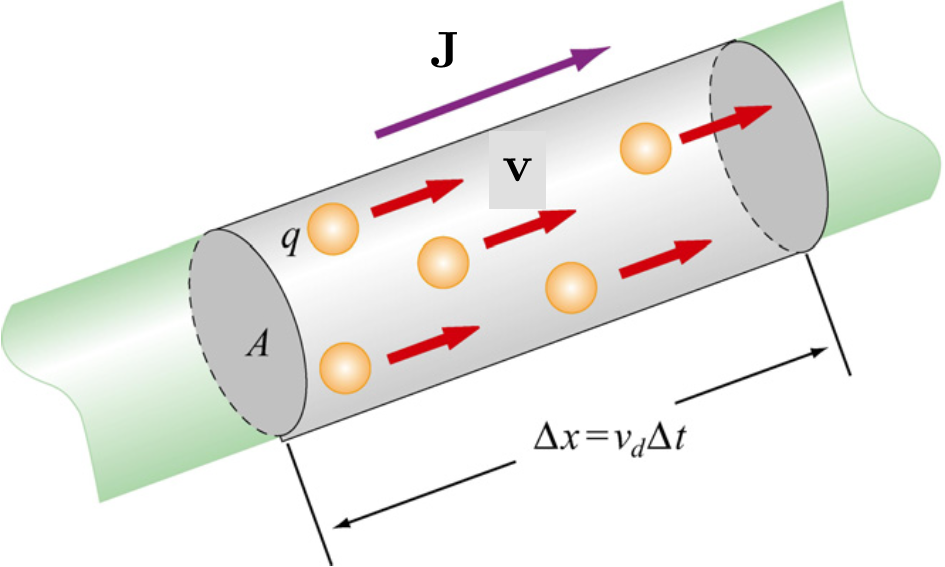
\includegraphics[scale=.3]{corrente_condutor}
\caption{\textit{Cargas elétrica fluindo no intervalo $\Delta\,x$ de um condutor com área de seção transversal $A$.}}
\label{fig.corre_condu}
\end{figure}
Observando a figura \ref{fig.corre_condu} que mostra uma corrente fluindo num condutor, onde $q$ é a carga elétrica de cada partícula, $n$ é quantidade de partículas num determinado volume do condutor e $\Delta\,x$ é o comprimento do mesmo, temos que a quantidade de carga nesse volume é $\Delta\,Q=n\,q\,(A\,\Delta\,x)$. Se as partículas se movem com velocidade $v$, então a posição a cada intervalo de tempo é dada por $\Delta\,x=v\,\Delta\,t$, e a corrente elétrica média nesse intervalo do condutor é
\begin{equation*}
I_m=\frac{\Delta\,Q}{\Delta\,t}=n\,q\,A\,v.
\end{equation*}
Como a densidade de corrente é a corrente média por área, temos que a mesma pode ser escrita como 
\begin{equation*}
\mathbf{J}=n\,q\,\mathbf{v}.
\end{equation*}

A terceira equação de Maxwell em sua forma integral pode ser obtida substituindo as equações \ref{eq.densidade_corrente} e \ref{eq.fluxo_eletrico} na equação \ref{eq.ampere_generalizada},
\begin{align*}
\int_s\mathbf{B}\cdot d\mathbf{s}&=\mu_0I+\mu_0\epsilon_0\frac{d\phi_E}{dt}\\
\int_s\frac{\mathbf{B}}{\mu_0}\cdot d\mathbf{s}&=\int\int_S\mathbf{J}\cdot\,d\mathbf{A}+\frac{d}{dt}\int\int_S\epsilon_0\,\textbf{E}\cdot\textit{d}\textbf{A}
\end{align*}

A quarta e última equação de Maxwell é obtida substituindo a equação do fluxo magnético \ref{eq.fluxo_mag} na lei de Faraday \ref{eq.lei_faraday},
\begin{align*}
\int_s\pmb{E}\cdot d\pmb{s}&=-\frac{d\phi_\mathbf{B}}{dt}\\
\int_s\pmb{E}\cdot d\pmb{s}&=-\frac{d}{dt}\int\int_S\pmb{B}\,d\pmb{A}.
\end{align*}

Todos os fenômenos eletromagnéticos são governados por essas quatro equações de Maxwell  e os últimos duzentos anos acumularam evidências suficientes para tal fato. Como vimos, todas as equações têm princípios experimentais, são deduzidas formalmente em termos de cálculo diferencial e integral, e são satisfeitas pelas variáveis físicas $\rho$ e $\mathbf{J}$ que são as fontes dos campos elétrico e magnético respectivamente. As equações são sumarizadas a seguir:
\begin{align*}
\int\int_S\epsilon_0\textbf{E}\cdot\textit{d}\textbf{A}&=\int\int\int_{V}\rho\,dV,\\\\
\int\int_S\textbf{B}\cdot\textit{d}\textbf{A}&=0,\\\\
\int_s\frac{\mathbf{B}}{\mu_0}\cdot d\mathbf{s}&=\int\int_S\mathbf{J}\cdot\,d\mathbf{A}+\frac{d}{dt}\int\int_S\epsilon_0\,\textbf{E}\cdot\textit{d}\textbf{A},\\\\
\int_s\pmb{E}\cdot d\pmb{s}&=-\frac{d}{dt}\int\int_S\pmb{B}\,d\pmb{A}.
\end{align*}

\section{Generalizações da teoria}

Nosso intuito é utilizar as equações de Maxwell para determinar a composição de uma determinada região da subsuperfície. As informaçãoes sobre as propriedades eletromagnéticas de uma região dependem dos parâmetros $\rho$ e $\mathbf{J}$ de cada região, e esses parâmetros são usados para definir e inserir nas equações de Maxwell dois campos vetoriais, $\mathbf{D}$ e $\mathbf{H}$, que estão diretamente ligados às características do meio como veremos a seguir.



\section{Conclusões}